\documentclass[12pt]{article}
\usepackage{latexsym}
\usepackage{amssymb,amsmath}
\usepackage[pdftex]{graphicx}
\usepackage{listings}
\usepackage{color}
\usepackage{graphicx}
\usepackage{caption}
\usepackage{subcaption}

\definecolor{dkgreen}{rgb}{0,0.6,0}
\definecolor{gray}{rgb}{0.5,0.5,0.5}
\definecolor{mauve}{rgb}{0.58,0,0.82}

\lstset{frame=tb,
  language=Java,
  aboveskip=3mm,
  belowskip=3mm,
  showstringspaces=false,
  columns=flexible,
  basicstyle={\small\ttfamily},
  numbers=none,
  numberstyle=\tiny\color{gray},
  keywordstyle=\color{blue},
  commentstyle=\color{dkgreen},
  stringstyle=\color{mauve},
  breaklines=true,
  breakatwhitespace=true,
  tabsize=3
}

\topmargin = 0.1in \textwidth=5.7in \textheight=8.6in

\oddsidemargin = 0.2in \evensidemargin = 0.2in


\begin{document}

\title{Experimentation with Clustering Algorithms}

\author{Corinne Curcie and Shivam Naik}
\date{March 5, 2017}

\maketitle

\begin{abstract}
Clustering algorithms are a popular tool for making sense of big data. Our project involved implementing various algorithms, focusing specifcally on high-dimensional data, to gain better understanding . 
\end{abstract}


\begin{enumerate}

\item Introduction

\item Related Work

\item Algorithms Implemented

\textbf{3.1 K-Means}

One of the algorithms we implemented is a variant on K-Means. Before getting into the details of that algorithm, we will go over the basics of K-Means, since we also used it as a benchmark when scoring preformances of algorithms we implemented. The well-known K-Means algorithm starts by choosing $k$ points in the dataset to be the initial cluster center points, and then updates on an ``expectation-maximization mechanism'' (EM).\\
 The ``E-step'' is the cluster assignment step, where points are labelled with a cluster based on which of the center points they are closest to. The ``M-step'' is the update step, where the $k$ cluster center points are recalculated to be some average of all of the points that were labeled as belonging to that cluster during the previous ``E-step'' round. The algorithm stops when the change in centers from one round to the next is less than some predetermined threshold. The objective function that K-Means tries to minimize is the sum of squared Euclidean distances from each point to its assigned cluster center:

$$ {\underset {\mathbf {S} }{\operatorname {arg\,min} }}\sum _{i=1}^{k}\sum _{\mathbf {x} \in S_{i}}\left\|\mathbf {x} -{\boldsymbol {\mu }}_{i}\right\|^{2} $$

\textbf{3.2 K-Subspaces}

We were intrigued by a 2009 paper that proposed a ``K-Subspaces" algorithm similar to K-Means (Wang, Ding, and Li 2009). Instead of using Euclidean distances for our objective function, multiple distance measures are used during the ``E-step'' to determine which centers the points are closest to. The authors of the algorithm decided to focus on three possible subspaces -- 1D lines, 2D planes, and 3D spheres -- and determines distance functions based on those subspaces. By calculating all three distances for each pair of point and cluster center, the algorithm is better able to determine when a point is within a cluster of a non-standard space. To extend this performance not only to the entire dataset but also subspaces within the dataset, PCA is used during distance calculations to isolate meaningful subspaces

\textbf{K-Subspaces Initialization} 

For initializing cluster centers before beginning the EM steps, we used the standard ``K-means++'' algorithm, which probabilistically selects initial clusters. Specifically, the algorithm goes through the following steps: (1) Select an input data point uniformly at random to be the first center. (2) Calculate the distance between every point $x$ and its nearest center point that has already been chosen. (3) Select a new data point as a next center, using a probability distribution where a point is chosen with probability proportional to the distance calculated in step 2. (4) Repeat the steps 2 and 3 until $k$ centers have been chosen. The ``K-means++'' initialization is also used in scikit-learn’s implementation of K-Means.

\textbf{Cluster Assignment Step}

In our cluster assignment step is when we use the new distance measures proposed by the authors. Instead of finding the direct distance to the center of a cluster, they aim to estimate a $\textit{surface}$ of a cluster by using perpendicular distances. For the following equations, let $x$ be a point and $C_k$ represent a cluster where $c_k$ is the center point of the cluster. 

\smallskip
\textbf{Line Distance:}

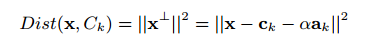
\includegraphics[scale=0.75]{eq1.png}

where

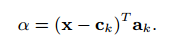
\includegraphics[scale=0.75]{eq12.png}

Here, $a_k$ represents the first principal component vector found using PCA.

\textbf{Plane Distance:}

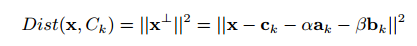
\includegraphics[scale=0.75]{eq2.png}

where 

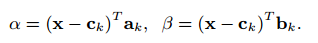
\includegraphics[scale=0.75]{eq22.png}

Here, $a_k$ again represents the first principal component vector found using PCA, and $b_k$ is the second principal component.

\smallskip

\textbf{Sphere Distance:}

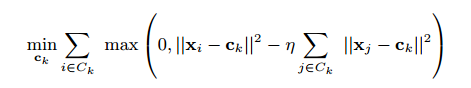
\includegraphics[scale=0.75]{eq3.png}




\textbf{DBScan}

DBScan stands for  Density-Based Algorithm for Discovering Clusters and was proposed by Martin Ester, Hans-Peter Kriegel, Jiirg Sander, Xiaowei Xu in 1996. The algorithm tries to find different clusters in the data based on two main parameters which are epsilon, the threshold for distance between two points, and min points, which is the threshold for minimum number of points required for a cluster. The samples from the dataset are classified in the clusters under 3 types of points: core points, border points, and noise points. Core points are within the epsilon of a center point, border points lie on the edges and can be flipped  to either of the close clusters, and noise points, which don’t belong to any clusters. The clusters are created by finding points closest to each other. We start with one point and find all the clusters closest to it and then find all the points closest to that cluster.

The algorithm:
We have a list of cluster id’s which is how we keep track of which sample belongs to which cluster. We go through each point and if it hasn’t been classified yet, then we “ExpandCluster”. Expand points starts by checking to see whether the current sample has at least min points number of neighbors by checking to see if the distance between the two samples is less than epsilon. If it fails to have enough neighbors with a short distance, all points are marked as NOISE. Otherwise, it goes through all the neighbors and finds all the points that it can reach to swallow into this its cluster by marking all cluster id’s as the same.

How to determine eps:
Find the k nearest(for our purposes 3) points and get the distance. Sort all distances and set the eps to the midway point. Will keep min points set to 4 according to the paper even though our data has a higher dimension than 2.

\textbf{Single Link Hierarchical Clustering}

Hierarchical clustering algorithms are used to cluster samples in a hierarchy leading to a dendrogram. Hierarchical clustering algorithms can either be agglomerative or divisive. Agglomerative Hierarchical Clustering starts by bucketing each sample in its own cluster and then merging two samples based on distance. Divisive Hierarchical Clustering starts by having all the samples in one cluster and splitting off the farthest sample in each step until each sample is in its own bucket.

For the purposes of our paper, we focused on agglomerative instead of divisive.  There are a few ways in which agglomerative clustering calculates which samples belong in a cluster together. They include complete linkage, single linkage, and average linkage. In complete linkage, the maximum between a sample from cluster a and cluster b is kept. Once largest maximum is calculated across all combinations of clusters, the two clusters are combined. In single linkage, the minimum between two points of two clusters is kept and the two clusters with the minimum distance from all combinations are combined. In average linkage, the average distance across all the points in each cluster is calculated and the clusters with the mean distance are combined. For the purposes of our project, we will use Single Linkage Hierarchical Clustering.

The Algorithm:
The algorithm starts by assigning a cluster id to each sample. We go through each of the clusters, which starts as an array of length N of one dimensional arrays consisting of the assigned cluster id. Once we find the min distance, we combine merge the second sample’s cluster id into the array holding the first sample’s cluster id. We keep doing this until we hit the max cluster level which we provide. This is a little tweak from the ful hierarchical clustering algorithm which stops when all the samples are in one cluster.

\begin{verbatim}

    def regionQuery(self, dataMatrix, pointIndex, eps):
        neighbors = []
        for i in xrange(len(dataMatrix)):
            if (self.dist(dataMatrix[i], dataMatrix[pointIndex]) <= eps):
                neighbors.append(i)
        neighbors.remove(pointIndex)
        return neighbors

    def expandCluster(self, dataMatrix, neighbors, eps, minPoints, clusters, pointIndex, clusterIndex):
        clusters[pointIndex] = clusterIndex
        for neighbors_iter in neighbors:
            if(clusters[neighbors_iter] < 0):
                clusters[neighbors_iter] = clusterIndex
                neighbors_2 = self.regionQuery(dataMatrix, neighbors_iter, eps)
                if(len(neighbors_2) > minPoints):
                    neighbors.extend(neighbors_2)

    def calculateEps(self, dataMatrix):
        neigh = NearestNeighbors(5, 1)
        neigh.fit(dataMatrix)
        kNearestDist =  (neigh.kneighbors(dataMatrix, 3, return_distance=True)[0]).flatten()
        sortedDistance = sorted(kNearestDist[kNearestDist != 0])
        return sortedDistance[len(sortedDistance)/2]

    def run_dbscan(self, dataMatrix, eps, minPoints):
        clusterIndex = 0
        clusters = [NOTVISITED] * len(dataMatrix)

        for i in xrange(len(dataMatrix)):
            if clusters[i] >= 0:
                continue
            neighbors = self.regionQuery(dataMatrix, i, eps)
            if(len(neighbors) < minPoints):
                for i in neighbors:
                    clusters[i] = NOISE
                continue
            else:
                self.expandCluster(dataMatrix, neighbors, eps, minPoints, clusters, i, clusterIndex)
                clusterIndex+=1
        return clusters

\end{verbatim}

\textbf{Single Link Hierarchical Clustering}

Hierarchical clustering algorithms are used to cluster samples in a hierarchy leading to a dendrogram. Hierarchical clustering algorithms can either be agglomerative or divisive. Agglomerative Hierarchical Clustering starts by bucketing each sample in its own cluster and then merging two samples based on distance. Divisive Hierarchical Clustering starts by having all the samples in one cluster and splitting off the farthest sample in each step until each sample is in its own bucket.

For the purposes of our paper, we focused on agglomerative instead of divisive.  There are a few ways in which agglomerative clustering calculates which samples belong in a cluster together. They include complete linkage, single linkage, and average linkage. In complete linkage, the maximum between a sample from cluster a and cluster b is kept. Once largest maximum is calculated across all combinations of clusters, the two clusters are combined. In single linkage, the minimum between two points of two clusters is kept and the two clusters with the minimum distance from all combinations are combined. In average linkage, the average distance across all the points in each cluster is calculated and the clusters with the mean distance are combined. For the purposes of our project, we will use Single Linkage Hierarchical Clustering.

The Algorithm:
The algorithm starts by assigning a cluster id to each sample. We go through each of the clusters, which starts as an array of length N of one dimensional arrays consisting of the assigned cluster id. Once we find the min distance, we combine merge the second sample’s cluster id into the array holding the first sample’s cluster id. We keep doing this until we hit the max cluster level which we provide. This is a little tweak from the ful hierarchical clustering algorithm which stops when all the samples are in one cluster.


\begin{verbatim}

    def calculateDistance(self, sample_a, sample_b):
        sum = 0
        for i in xrange(len(sample_a)):
            sum += (math.pow(sample_a[i]-sample_b[i], 2))
        return math.sqrt(sum)

    def mergeClusters(self, clusters, index_1, index_2):
        clusters[index_1].extend(clusters[index_2])
        del clusters[index_2]
        return clusters

    def runAggClustering(self, X, cluster_level = 1):
        clusters = [[index] for index in range(0, len(X))]
        while(len(clusters) > cluster_level):
            indicies = (-1, -1)
            minDistance = float("Inf")

            for i in xrange(len(clusters)):
                for j in xrange(i+1, len(clusters)):
                    if(i==j):
                        continue
                    for index_i in clusters[i]:
                        for index_j in clusters[j]:
                            distance = self.calculateDistance(X[index_i], X[index_j])
                            if(distance < minDistance):
                                minDistance = distance
                                indicies = (i,j)

            self.mergeClusters(clusters, indicies[0], indicies[1])
        return clusters

\end{verbatim}

\item Datasets Used

\item Performance

\textbf{K-Subspaces on Synthetic Data}

For our synthetic data, we ran a very similar synthetic experiment to the one presented in the 2009 paper. We wanted to demonstrate the ability of K-subspaces to cluster for a variety of shapes. Data includes 1D lines, 2D planes, and 3D spheres, and the goal is for K-Subspaces to cluster those shapes together separately even when they are close together. We are comparing the performance with scikit-learn's implementation of K-Means. 

\begin{figure}
    \centering
    \begin{subfigure}[b]{0.3\textwidth}
        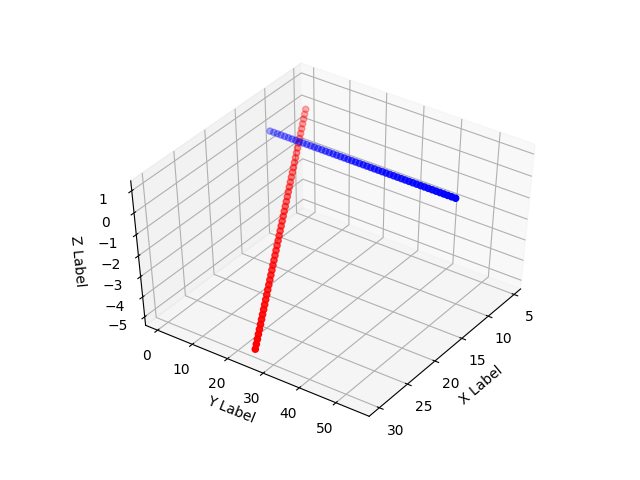
\includegraphics[width=\textwidth]{ksubfigures/2lines.png}
        \caption{Original Data}
        \label{fig:2lines}
    \end{subfigure}
    \begin{subfigure}[b]{0.3\textwidth}
        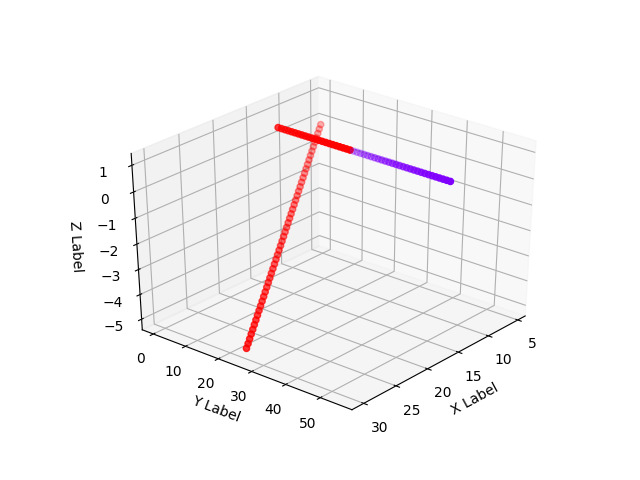
\includegraphics[width=\textwidth]{ksubfigures/2lineskmeans.png}
        \caption{K-Means}
        \label{fig:kmeans}
    \end{subfigure}
    ~ %add desired spacing between images, e. g. ~, \quad, \qquad, \hfill etc. 
    %(or a blank line to force the subfigure onto a new line)
    \begin{subfigure}[b]{0.3\textwidth}
        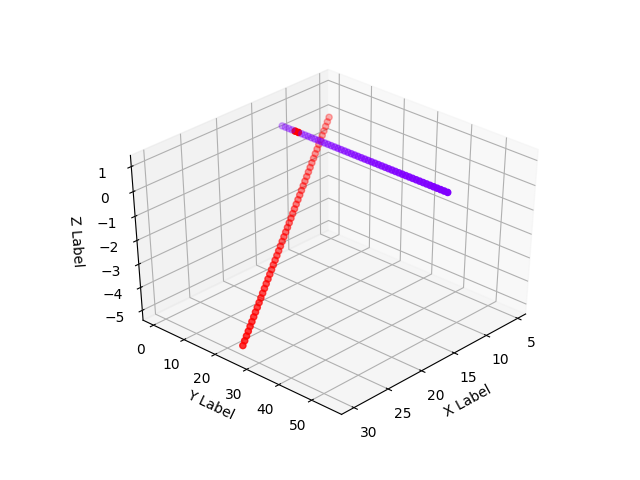
\includegraphics[width=\textwidth]{ksubfigures/2linesksub.png}
        \caption{K-Subspaces}
        \label{fig:ksub}
    \end{subfigure}
    \caption{Performance on two 1-D Subspaces}\label{fig:2lineswhole}
\end{figure}


\begin{figure}
    \centering
    \begin{subfigure}[b]{0.3\textwidth}
        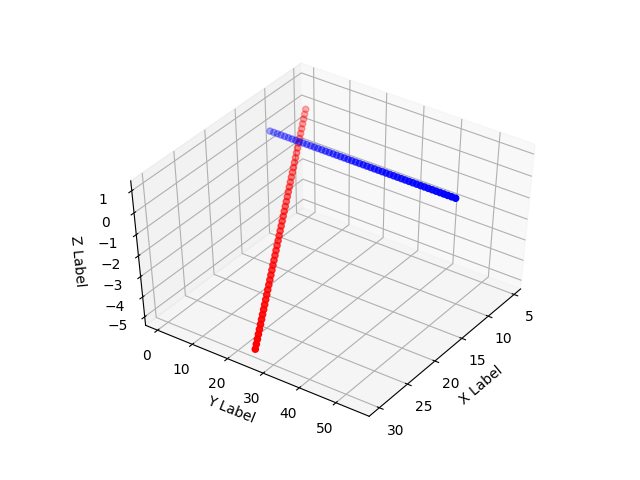
\includegraphics[width=\textwidth]{ksubfigures/2lines.png}
        \caption{Original Data}
        \label{fig:2lines}
    \end{subfigure}
    \begin{subfigure}[b]{0.3\textwidth}
        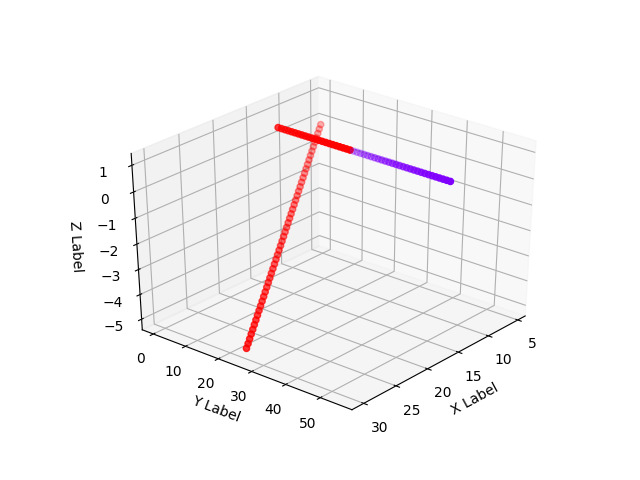
\includegraphics[width=\textwidth]{ksubfigures/2lineskmeans.png}
        \caption{K-Means}
        \label{fig:kmeans}
    \end{subfigure}
    ~ %add desired spacing between images, e. g. ~, \quad, \qquad, \hfill etc. 
    %(or a blank line to force the subfigure onto a new line)
    \begin{subfigure}[b]{0.3\textwidth}
        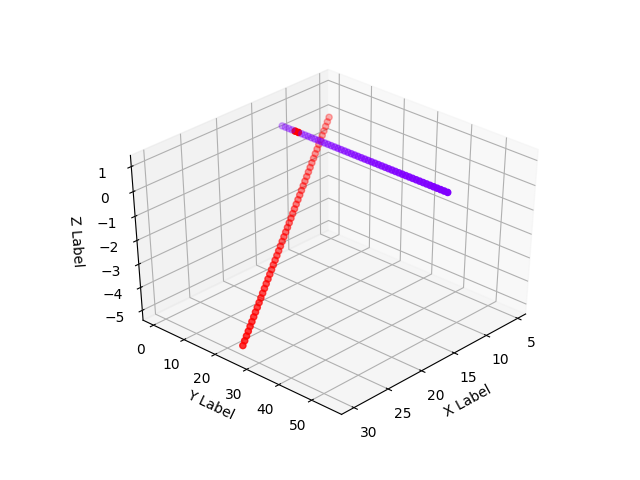
\includegraphics[width=\textwidth]{ksubfigures/2linesksub.png}
        \caption{K-Subspaces}
        \label{fig:ksub}
    \end{subfigure}
    \caption{Performance on two 1-D Subspaces}\label{fig:2lineswhole}
\end{figure}





\end{enumerate}

\end{document} 
